\subsection{Neural architecture}

\subsubsection{Structure}
The line
\begin{lstlisting}[language=Python]
    x = torch.cat((x_input, x), dim=1)
\end{lstlisting}
takes the original input \(\texttt{x\_input}\) (the raw state features) and concatenates it with the hidden representation \(\texttt{x}\) along the feature dimension. This effectively merges the initial state features with the learned features from the hidden layers. Such a design is sometimes referred to as a \emph{skip connection} or \emph{residual-like} connection, because the network has direct access to the original input when producing the final Q-values.

\subsubsection{Activation function}
We use \(\tanh\) instead of the standard logistic sigmoid function because:
\begin{itemize}
  \item \(\tanh\) is zero-centered (ranging from \(-1\) to \(1\)), which often helps with training stability.
  \item The logistic (sigmoid) function saturates more easily at 0 or 1, leading to slower gradients. In contrast, \(\tanh\) keeps activations in a range that often accelerates convergence in practice.
\end{itemize}

\subsection{Adding the Q-learning}
The missing line to compute the target \(\mathbf{y}\) (right after the comment ``\texttt{\# Compute targets}'') is shown below. We also detach the tensor so that the gradient does not flow back through the next-state values:

\begin{lstlisting}[language=Python]
    max_elements = torch.max(target_Qs, dim=1)[0].detach()
    y = rewards + gamma * max_elements
\end{lstlisting}

This implements the standard Q-learning target:
\[
y_i \;=\; r_i \;+\; \gamma \,\max_{a'}Q(s'_i,\;a').
\]
After adding this line, the training converged to policies achieving returns above 200 in many episodes, indicating that the agent successfully learned to land.

\subsubsection*{Learning curve}
\begin{figure}[H]
  \centering
  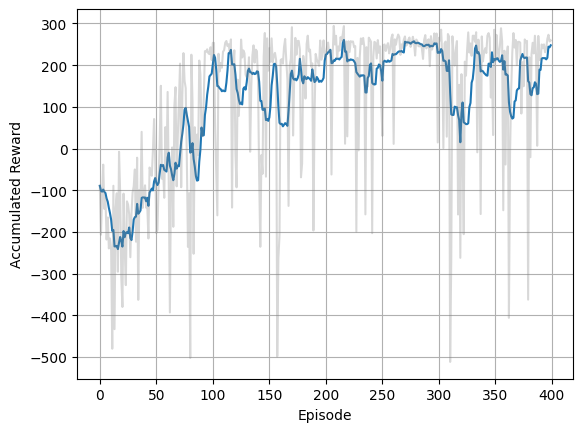
\includegraphics[width=0.65\textwidth]{Code/output.png}
  \caption{Accumulated reward per episode (in gray) and its smoothed average (blue).}
\end{figure}

\subsection{Epsilon}
The line
\begin{lstlisting}[language=Python]
    explore_p = explore_stop + (explore_start - explore_stop)*np.exp(-decay_rate*ep)
\end{lstlisting}
implements an exponentially decaying exploration probability. At the beginning (when \(\texttt{ep} = 0\)), it starts near \(\texttt{explore\_start}\), and as the episode index \(\texttt{ep}\) grows, the probability \(\texttt{explore\_p}\) exponentially approaches \(\texttt{explore\_stop}\). This ensures that early in training the agent explores more, and then it gradually exploits its learned policy more often.

\subsection{Gather}
The line
\begin{lstlisting}[language=Python]
    Q_tensor = torch.gather(output_tensor, 1, actions_tensor.unsqueeze(-1)).squeeze()
\end{lstlisting}
selects the Q-value corresponding to the action actually taken in each state. Since \(\texttt{output\_tensor}\) contains Q-values for all possible actions, we use \(\texttt{gather}\) along the action dimension to pick out the one Q-value that corresponds to the \(\texttt{actions\_tensor}\). In other words, it is a convenient way to index a batch of Q-value vectors by their chosen actions.